\documentclass[a4paper]{article}

%%%%%%%%%%%%%%%%%%%%%%%%%%%%%%%%%%
% Package for making LaTeX properly handle utf8 characters set and danish language rules
\usepackage[utf8]{inputenc}
\usepackage[danish]{babel}

%%%%%%%%%%%%%%%%%%%%%%%%%%%%%%%%%%
% Package for changing to a nicer font 
\usepackage [T1]{fontenc}

%%%%%%%%%%%%%%%%%%%%%%%%%%%%%%%%%%
% Package for conctroling the text area
\usepackage[margin=2.5cm]{geometry}

%%%%%%%%%%%%%%%%%%%%%%%%%%%%%%%%%%
% Package for inserting clickable hyperlinks in pdf versions as produced by pdflatex
\usepackage{hyperref}

%%%%%%%%%%%%%%%%%%%%%%%%%%%%%%%%%%
% Package for including figures. TeX and thus LaTeX was developped before the existence of directory file-structures, but the graphicspath let's you add directories, that the \includegraphics will search.
\usepackage{graphicx}
\graphicspath{{figures/}{anotherFigureDirectory/}}

%%%%%%%%%%%%%%%%%%%%%%%%%%%%%%%%%%
% Package for typesetting programs. Listings does not support fsharp, but a little modification goes a long way
\usepackage{listings}
\usepackage{color}

\definecolor{bluekeywords}{rgb}{0.13,0.13,1}
\definecolor{greencomments}{rgb}{0,0.5,0}
\definecolor{turqusnumbers}{rgb}{0.17,0.57,0.69}
\definecolor{redstrings}{rgb}{0.5,0,0}

\lstdefinelanguage{FSharp}
                {morekeywords={let, new, match, with, rec, open, module, namespace, type, of, member, and, for, in, do, begin, end, fun, function, try, mutable, if, then, else},
    keywordstyle=\color{bluekeywords},
    sensitive=false,
    morecomment=[l][\color{greencomments}]{///},
    morecomment=[l][\color{greencomments}]{//},
    morecomment=[s][\color{greencomments}]{{(*}{*)}},
    morestring=[b]",
    stringstyle=\color{redstrings}
    }
%%%%%%%%%%%%%%%%%%%%%%%%%%%%%%%%%%
% Package for extended math settings, e.g. \eqref
\usepackage{amsmath}

%%%%%%%%%%%%%%%%%%%%%%%%%%%%%%%%%%
% These will be the title and author, as included when \maketitle is called.
\title{Rapportskabelon}
\author{Jon Sporring }

\begin{document}
\maketitle % Insert title etc.

% sections are the outer logical structure when using documentclass-article, while chapter would be the outer structure, when using report documentclass
\section{Forord}
Forordet omhandler selve rapporten. Forordet skal give læseren et billede af rammerne for rapporten. Forordet indeholder ofte:
% A bullet list
\begin{itemize}
\item Hvem har skrevet rapporten, hvornår og i hvilken forbindelse?
\item Hvordan er rapporten blevet til? Er den et eksamensprojekt, er der en opgavestiller og i fald hvem? Det vil også være naturligt at inkludere en evt. projektkontrakt her, hvis den ikke er lang.
\item Tak til vejledere, faglige hjælpere, og andre, som har bidraget til rapporten.
\end{itemize}
Forordet er et selvstændigt kapitel i rapporten og i en hvis forstand ikke en del af selve rapporten men mere et forklæde til rapporten. For korte rapporter er forordet ofte udeladt.

\section{Introduktion}
Dette afsnit skal give en indledning til rapportens emne på et overordnet plan. Introduktion skal typisk skrives, så den kan læses sammen med konklusionen med kun et overfladisk kendskab til resten af rapportens indhold. Indledningen indeholder en kort og overordnet introduktion til de faglige elementer, som rapporten omhandler, motivation for arbejdets udførsel, en kort opsummering af eksisterende arbejde med præcise referencer til litteraturen, og muligvis "`teasers"' for de resultater, som er opnået i arbejdet. Husk at en figur kan være meget illustrativ, når man vil give læseren en overordnet forståelse, se f.eks.\ Figur~\ref{fig:eksempel}.
% A floating figure. The \label is paired with \ref in the text. 
\begin{figure}
  \centering
  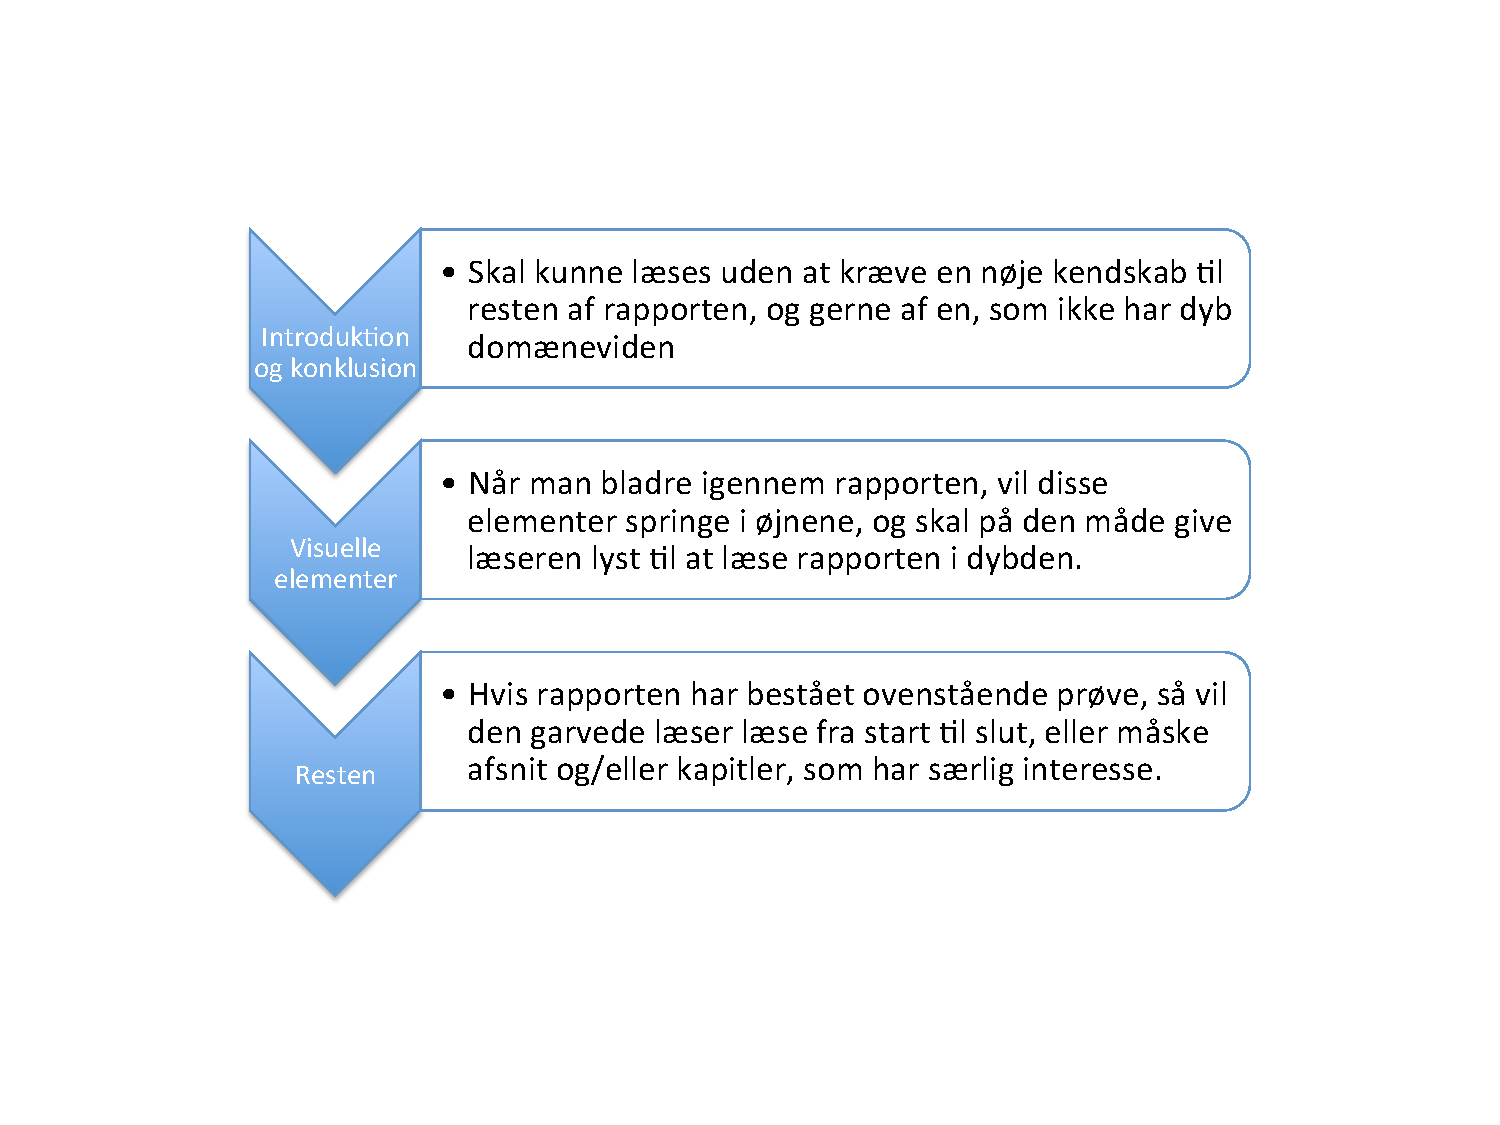
\includegraphics[width=0.6\linewidth]{Reading} % We don't need to specify the filename suffix
  \caption{En figur giver en mulighed for at kommunikere med visuelle virkemidler, som kan støtte læsningen. I figuren ses en opsummering af, hvordan en garvet læser ofte læser rapporter.}
  \label{fig:eksempel}
\end{figure}

\section{Problemformulering}
Kan slås sammen med indledning. Problemformuleringen indeholder typisk en præcis beskrivelse af det problem eller den hypotese, som rapporten omhandler. Dette vil også være et naturligt sted at beskrive hvilke afgrænsninger mht. problem domæne og løsningsrum, som man har gjort.

\section{Problemanalyse og design}
I dette afsnit beskrives den analyse, som man har gjort for at løse problemet. Det er vigtigt, at de løsningsmuligheder, der er blevet overvejet, beskrives, samt at man kommer med objektive begrundelser for de valg, som er gjort. Figurer af f.eks.\ programdesignet, er som regel at finde i dette afsnit. Dette afsnit indeholder ofte en overordnet beskrivelse af de centrale datastrukturer skitseres samt en skitse af de vigtigste (dele af) funktioner og deres typer.

\section{Programbeskrivelse}
Programbeskrivelsen er en gennemgang af det producerede program. De centrale problemstillinger med at omforme centrale valg for Problemanalysen til det konkrete program. Det vil ofte være naturligt kun at fokusere på ikke-oplagte løsninger og særlige indsigter og tricks, der er brugt. Eksempelvis kunne man inkludere programkode stumper som f.eks.\ vist i Figur~\ref{fig:fsharpCodeExample}
\begin{figure}
  \lstset{language=FSharp}
\begin{lstlisting}
(* Fibonacci Number formula *)
let rec fib n =
    match n with
    | 0 | 1 -> n
    | _ -> fib (n - 1) + fib (n - 2)
\end{lstlisting}
  \caption{An example of a program listing. Sometimes this is included in a float, other times inline in the text.}
  \label{fig:fsharpCodeExample}
\end{figure}


Programbeskrivelsen giver en kort beskrivelse af, hvordan programmet bruges. F.eks.\ hvis programmet skal køres fra kommandolinjen, hvilke argumenter kan benyttes og hvad er deres effekt. 


\section{Afprøvning og eksperimenter}
Afprøvningens formål er at dokumentere det udviklede programs korrekthed ved at forfatteren/forfatterne har designet et sæt af tekstkørsler. Hvis der er tale om et mere eksperimentelt arbejde, hvor en grundig gennemgang af inputdomæne ikke er muligt, vil afsnittet også indeholde en beskrivelse af og resultatet af et sæt af eksperimenter, som sandsynliggør i hvilken grad programmet løser Problemformuleringen. Hvis man f.eks.\ ønsker at dokumentere køretider, vil det være naturligt at lave realistiske eksperimenter, hvor programmet køres på forskellig data.

Det er vigtigt at huske at beskrive, efter hvilke principper afprøvningen og eksperimenterne er blevet designet, og at argumentere for i hvilken grad de dækker det relevante problemområde og i hvor høj grad de viser, at programmet løser Problemformuleringen. Dette afsnit vil ofte drage delkonklusioner, som opsummeres i konklusionsafsnittet.

\section{Diskussion og konklusion}
Diskussion og konklusionsafsnittet opsummerer problemstillingen, gennemgår de resultater, der er opnået. Dette afsnit skal også på kort og præcis form beskrive, om evt. i hvor høj grad Problemformuleringen er løst. Dette afsnit skal også indeholde reflektioner over valg, opsummering af, hvad man har lært i processen, og kan indeholde forslag til videre arbejde.

Husk at dette afsnit oftest læses først, lige efter introduktionen, og den skal derfor kunne fungere uden detaljeret kendskab til de mellemlæggende afsnit.

\section{Efterskrift}
Ofte indeholder videnskabelige arbejder ikke et efterskrift, men i denne korte oversigt vil efterskriftet blive brugt til at liste generelle råd til rapportskrivning:
\begin{itemize}
\item Husk det er din opgave at sikre at dine ideer og tanker bliver kommunikeret til læseren. At det højst sandsynligt er første gang, læseren ser din tekst og figurer, og du derfor ikke kan antage, at læseren kan gætte, hvad du måske finder oplagt.
\item En typisk rækkefølge, som en garvet læser læser rapporter er: 1) Introduktion og Konklusion, 2) Bladre igennem rapporten og kigge på figurerne og centrale visuelle elementer som en tegneserie, 3) Læse rapporten fra forside til bagside. Det kan anbefales, at man prøver at kigge på sin rapport med lignende briller.
\item Introduktion og konklusioner er første bastion, som ofte afgør om læseren vil fortsætte læsning (med glæde). De er ofte de afsnit, som skrives sidst, da det indre af rapporten ofte udvikler sig indtil sidste, og da det er derfor vigtigt at vente med en færdigskrivning, så alt kommer med.
\item Husk at alle grafiske elementer, som benyttes i figuren skal beskrives i figurteksten inkl.\ f.eks.\ en beskrivelse af aksers enheder og hvad graferne viser, at der er tale om pseudokode, eller at det er et uml diagram, etc.. Husk at læseren sandsynligvis ser figurerne for første gang, og derfor ikke har samme antagelser eller synes at de samme ting er oplagte som forfatteren.
\item Som skribent oplever man ofte en blindhed overfor sin produktion: Når man læser, hvad man har skrevet, overser man fejl og mangler og i stedet læser, hvad der burde have stået. En simpel måde, at sikre at rapport bliver en fornøjelse at læse er Læse Højt metoden. Metodens formål er at sikre, at sætninger kan læses og argumenter kommer i en logisk rækkefølge.  Metoden er som følger: Bed en læse central afsnit højt for dig, og noter dig, hvilke steder i teksten, højtlæsningen går i stå eller på anden vis giver højtlæseren problemer. For afsnit som f.eks.\ introduktion og konklusion behøver højtlæseren ikke at have domæneviden, da disse afsnit ofte skal skrives så udenforstående kan få noget ud af at læse dem.
\item Et klikbart links kan indsættes med hyperlink pakken og pdflatex: \url{https://www.ctan.org}.
\end{itemize}


\end{document}

